
\columnratio{0.55}
\begin{paracol}{2} 
 
\switchcolumn[0]*%%%%%%%
\section{Rendering Mechanism}
\switchcolumn
\section{渲染机制}
\switchcolumn[0]*%%%%%%%
How does Vue take a template and turn it into actual DOM nodes? How does
Vue update those DOM nodes efficiently? We will attempt to shed some
light on these questions here by diving into Vue's internal rendering
mechanism.
\switchcolumn
Vue 是如何将一份模板转换为真实的 DOM
节点的,又是如何高效地更新这些节点的呢?我们接下来就将尝试通过深入研究
Vue 的内部渲染机制来解释这些问题。
\switchcolumn[0]*%%%%%%%
\subsection{Virtual DOM}
\switchcolumn
\subsection{虚拟 DOM}
\switchcolumn[0]*%%%%%%%
You have probably heard about the term "virtual DOM", which Vue's
rendering system is based upon.
\switchcolumn
你可能已经听说过``虚拟 DOM''的概念了,Vue
的渲染系统正是基于这个概念构建的。
\switchcolumn[0]*%%%%%%%
The virtual DOM (VDOM) is a programming concept where an ideal, or
``virtual'', representation of a UI is kept in memory and synced with
the ``real'' DOM. The concept was pioneered by
\href{https://reactjs.org/}{React}, and has been adopted in many other
frameworks with different implementations, including Vue.
\switchcolumn
虚拟 DOM (Virtual DOM,简称 VDOM) 是一种编程概念,意为将目标所需的 UI
通过数据结构``虚拟''地表示出来,保存在内存中,然后将真实的 DOM
与之保持同步。这个概念是由 \href{https://reactjs.org/}{React}
率先开拓,随后被许多不同的框架采用,当然也包括 Vue。
\switchcolumn[0]*%%%%%%%
Virtual DOM is more of a pattern than a specific technology, so there is
no one canonical implementation. We can illustrate the idea using a
simple example:
\switchcolumn
与其说虚拟 DOM
是一种具体的技术,不如说是一种模式,所以并没有一个标准的实现。我们可以用一个简单的例子来说明:
\switchcolumn[0]*%%%%%%%
\begin{codeJs}
const vnode = {
  type: 'div',
  props: {
    id: 'hello'
  },
  children: [
    /* 更多 vnode */
  ]
}
\end{codeJs}
\switchcolumn
\begin{codeJs}
const vnode = {
  type: 'div',
  props: {
    id: 'hello'
  },
  children: [
    /* 更多 vnode */
  ]
}
\end{codeJs}
\switchcolumn[0]*%%%%%%%
Here, \texttt{vnode} is a plain JavaScript object (a "virtual node")
representing a \texttt{\textless{}div\textgreater{}} element. It
contains all the information that we need to create the actual element.
It also contains more children vnodes, which makes it the root of a
virtual DOM tree.
\switchcolumn
这里所说的 \texttt{vnode} 即一个纯 JavaScript 的对象
(一个``虚拟节点''),它代表着一个 \texttt{\textless{}div\textgreater{}}
元素。它包含我们创建实际元素所需的所有信息。它还包含更多的子节点,这使它成为虚拟
DOM 树的根节点。
\switchcolumn[0]*%%%%%%%
A runtime renderer can walk a virtual DOM tree and construct a real DOM
tree from it. This process is called \textbf{mount}.
\switchcolumn
一个运行时渲染器将会遍历整个虚拟 DOM 树,并据此构建真实的 DOM
树。这个过程被称为\textbf{挂载} (mount)。
\switchcolumn[0]*%%%%%%%
If we have two copies of virtual DOM trees, the renderer can also walk
and compare the two trees, figuring out the differences, and apply those
changes to the actual DOM. This process is called \textbf{patch}, also
known as "diffing" or "reconciliation".
\switchcolumn
如果我们有两份虚拟 DOM
树,渲染器将会有比较地遍历它们,找出它们之间的区别,并应用这其中的变化到真实的
DOM 上。这个过程被称为\textbf{更新} (patch),又被称为``比对''(diffing)
或``协调''(reconciliation)。
\switchcolumn[0]*%%%%%%%
The main benefit of virtual DOM is that it gives the developer the
ability to programmatically create, inspect and compose desired UI
structures in a declarative way, while leaving the direct DOM
manipulation to the renderer.
\switchcolumn
虚拟 DOM
带来的主要收益是它让开发者能够灵活、声明式地创建、检查和组合所需 UI
的结构,同时只需把具体的 DOM 操作留给渲染器去处理。
\end{paracol}



\columnratio{0.55}
\begin{paracol}{2} 
 
\switchcolumn[0]*%%%%%%%
\subsection{Render Pipeline}
\switchcolumn
\subsection{渲染管线}
\switchcolumn[0]*%%%%%%%
At the high level, this is what happens when a Vue component is mounted:
\switchcolumn
从高层面的视角看,Vue 组件挂载时会发生如下几件事:
\switchcolumn[0]*%%%%%%%
\begin{enumerate}
\item
  \textbf{Compile}: Vue templates are compiled into \textbf{render
  functions}: functions that return virtual DOM trees. This step can be
  done either ahead-of-time via a build step, or on-the-fly by using the
  runtime compiler.
\item
  \textbf{Mount}: The runtime renderer invokes the render functions,
  walks the returned virtual DOM tree, and creates actual DOM nodes
  based on it. This step is performed as a
  \href{https://vuejs.org/guide/extras/reactivity-in-depth.html}{reactive
  effect}, so it keeps track of all reactive dependencies that were
  used.
\item
  \textbf{Patch}: When a dependency used during mount changes, the
  effect re-runs. This time, a new, updated Virtual DOM tree is created.
  The runtime renderer walks the new tree, compares it with the old one,
  and applies necessary updates to the actual DOM.
\end{enumerate}
\switchcolumn
\begin{enumerate}
\item
  \textbf{编译}:Vue 模板被编译为\textbf{渲染函数}:即用来返回虚拟 DOM
  树的函数。这一步骤可以通过构建步骤提前完成,也可以通过使用运行时编译器即时完成。
\item
  \textbf{挂载}:运行时渲染器调用渲染函数,遍历返回的虚拟 DOM
  树,并基于它创建实际的 DOM
  节点。这一步会作为\href{https://cn.vuejs.org/guide/extras/reactivity-in-depth.html}{响应式副作用}执行,因此它会追踪其中所用到的所有响应式依赖。
\item
  \textbf{更新}:当一个依赖发生变化后,副作用会重新运行,这时候会创建一个更新后的虚拟
  DOM
  树。运行时渲染器遍历这棵新树,将它与旧树进行比较,然后将必要的更新应用到真实
  DOM 上去。
\end{enumerate}
\end{paracol}

\begin{center} 
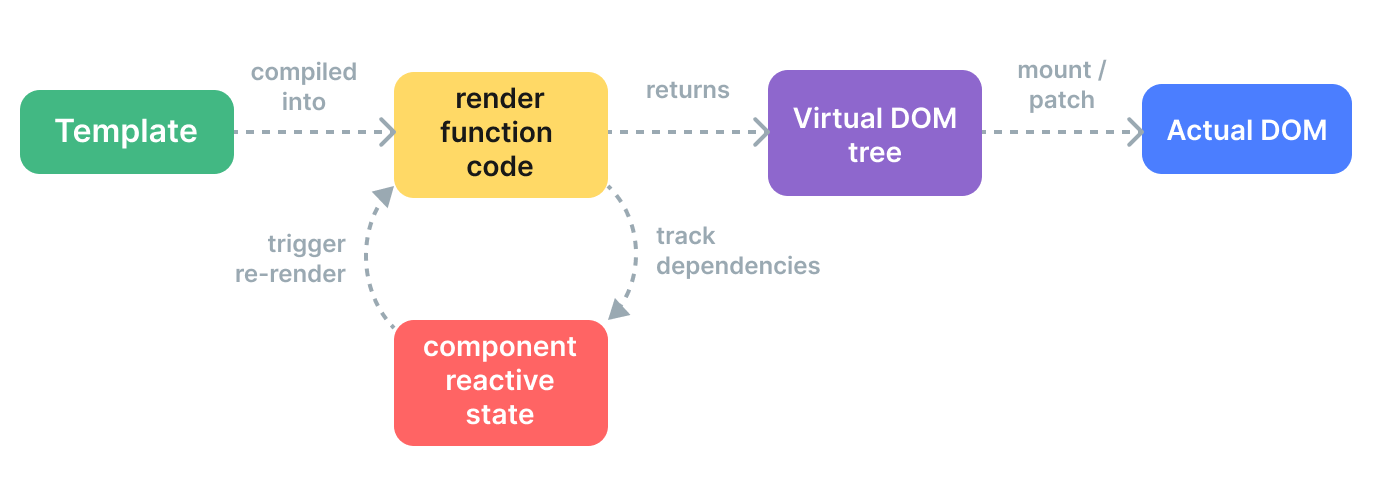
\includegraphics{./img/render-pipeline.03805016.png} 
\end{center}
    

\columnratio{0.55}
\begin{paracol}{2} 
 
\switchcolumn[0]*%%%%%%%
\subsection{Templates vs. Render Functions}
\switchcolumn
\subsection{模板 vs. 渲染函数}
\switchcolumn[0]*%%%%%%%
Vue templates are compiled into virtual DOM render functions. Vue also
provides APIs that allow us to skip the template compilation step and
directly author render functions. Render functions are more flexible
than templates when dealing with highly dynamic logic, because you can
work with vnodes using the full power of JavaScript.
\switchcolumn
Vue 模板会被预编译成虚拟 DOM 渲染函数。Vue 也提供了 API
使我们可以不使用模板编译,直接手写渲染函数。在处理高度动态的逻辑时,渲染函数相比于模板更加灵活,因为你可以完全地使用
JavaScript 来构造你想要的 vnode。
\switchcolumn[0]*%%%%%%%
So why does Vue recommend templates by default? There are a number of
reasons:
\switchcolumn
那么为什么 Vue 默认推荐使用模板呢?有以下几点原因:
\switchcolumn[0]*%%%%%%%
\begin{enumerate}
\def\labelenumi{\arabic{enumi}.}
\item
  Templates are closer to actual HTML. This makes it easier to reuse
  existing HTML snippets, apply accessibility best practices, style with
  CSS, and for designers to understand and modify.
\item
  Templates are easier to statically analyze due to their more
  deterministic syntax. This allows Vue's template compiler to apply
  many compile-time optimizations to improve the performance of the
  virtual DOM (which we will discuss below).
\end{enumerate}
\switchcolumn
\begin{enumerate}
\def\labelenumi{\arabic{enumi}.}
\item
  模板更贴近实际的 HTML。这使得我们能够更方便地重用一些已有的 HTML
  代码片段,能够带来更好的可访问性体验、能更方便地使用 CSS
  应用样式,并且更容易使设计师理解和修改。
\item
  由于其确定的语法,更容易对模板做静态分析。这使得 Vue
  的模板编译器能够应用许多编译时优化来提升虚拟 DOM 的性能表现
  (下面我们将展开讨论)。
\end{enumerate}
\switchcolumn[0]*%%%%%%%
In practice, templates are sufficient for most use cases in
applications. Render functions are typically only used in reusable
components that need to deal with highly dynamic rendering logic. Render
function usage is discussed in more detail in
\href{https://vuejs.org/guide/extras/render-function.html}{Render
Functions \& JSX}.
\switchcolumn
在实践中,模板对大多数的应用场景都是够用且高效的。渲染函数一般只会在需要处理高度动态渲染逻辑的可重用组件中使用。想了解渲染函数的更多使用细节可以去到\href{https://cn.vuejs.org/guide/extras/render-function.html}{渲染函数
\& JSX} 章节继续阅读。
\switchcolumn[0]*%%%%%%%
\subsection{Compiler-Informed Virtual DOM}
\switchcolumn
\subsection{带编译时信息的虚拟 DOM}
\switchcolumn[0]*%%%%%%%
The virtual DOM implementation in React and most other virtual-DOM
implementations are purely runtime: the reconciliation algorithm cannot
make any assumptions about the incoming virtual DOM tree, so it has to
fully traverse the tree and diff the props of every vnode in order to
ensure correctness. In addition, even if a part of the tree never
changes, new vnodes are always created for them on each re-render,
resulting in unnecessary memory pressure. This is one of the most
criticized aspect of virtual DOM: the somewhat brute-force
reconciliation process sacrifices efficiency in return for
declarativeness and correctness.
\switchcolumn
虚拟 DOM 在 React
和大多数其他实现中都是纯运行时的:更新算法无法预知新的虚拟 DOM
树会是怎样,因此它总是需要遍历整棵树、比较每个 vnode 上 props
的区别来确保正确性。另外,即使一棵树的某个部分从未改变,还是会在每次重渲染时创建新的
vnode,带来了大量不必要的内存压力。这也是虚拟 DOM
最受诟病的地方之一:这种有点暴力的更新过程通过牺牲效率来换取声明式的写法和最终的正确性。
\switchcolumn[0]*%%%%%%%
But it doesn't have to be that way. In Vue, the framework controls both
the compiler and the runtime. This allows us to implement many
compile-time optimizations that only a tightly-coupled renderer can take
advantage of. The compiler can statically analyze the template and leave
hints in the generated code so that the runtime can take shortcuts
whenever possible. At the same time, we still preserve the capability
for the user to drop down to the render function layer for more direct
control in edge cases. We call this hybrid approach
\textbf{Compiler-Informed Virtual DOM}.
\switchcolumn
但实际上我们并不需要这样。在 Vue
中,框架同时控制着编译器和运行时。这使得我们可以为紧密耦合的模板渲染器应用许多编译时优化。编译器可以静态分析模板并在生成的代码中留下标记,使得运行时尽可能地走捷径。与此同时,我们仍旧保留了边界情况时用户想要使用底层渲染函数的能力。我们称这种混合解决方案为\textbf{带编译时信息的虚拟
DOM}。
\switchcolumn[0]*%%%%%%%
Below, we will discuss a few major optimizations done by the Vue
template compiler to improve the virtual DOM's runtime performance.
\switchcolumn
下面,我们将讨论一些 Vue 编译器用来提高虚拟 DOM 运行时性能的主要优化:
\switchcolumn[0]*%%%%%%%
\subsubsection{Static Hoisting}
\switchcolumn
\subsubsection{静态提升}
\switchcolumn[0]*%%%%%%%
Quite often there will be parts in a template that do not contain any
dynamic bindings:
\switchcolumn
在模板中常常有部分内容是不带任何动态绑定的:
\switchcolumn[0]*%%%%%%%
\begin{codeHtml}
<div>
  <div>foo</div> <!-- 需提升 -->
  <div>bar</div> <!-- 需提升 -->
  <div>{{ dynamic }}</div>
</div>
\end{codeHtml}
\switchcolumn
\begin{codeHtml}
<div>
  <div>foo</div> <!-- 需提升 -->
  <div>bar</div> <!-- 需提升 -->
  <div>{{ dynamic }}</div>
</div>
\end{codeHtml}
\switchcolumn[0]*%%%%%%%
\href{https://template-explorer.vuejs.org/\#eyJzcmMiOiI8ZGl2PlxuICA8ZGl2PmZvbzwvZGl2PiA8IS0tIGhvaXN0ZWQgLS0+XG4gIDxkaXY+YmFyPC9kaXY+IDwhLS0gaG9pc3RlZCAtLT5cbiAgPGRpdj57eyBkeW5hbWljIH19PC9kaXY+XG48L2Rpdj5cbiIsIm9wdGlvbnMiOnsiaG9pc3RTdGF0aWMiOnRydWV9fQ==}{Inspect
in Template Explorer}
\switchcolumn
\href{https://template-explorer.vuejs.org/\#eyJzcmMiOiI8ZGl2PlxuICA8ZGl2PmZvbzwvZGl2PiA8IS0tIGhvaXN0ZWQgLS0+XG4gIDxkaXY+YmFyPC9kaXY+IDwhLS0gaG9pc3RlZCAtLT5cbiAgPGRpdj57eyBkeW5hbWljIH19PC9kaXY+XG48L2Rpdj5cbiIsIm9wdGlvbnMiOnsiaG9pc3RTdGF0aWMiOnRydWV9fQ==}{在模板编译预览中查看}
\switchcolumn[0]*%%%%%%%
The \texttt{foo} and \texttt{bar} divs are static - re-creating vnodes
and diffing them on each re-render is unnecessary. The Vue compiler
automatically hoists their vnode creation calls out of the render
function, and reuses the same vnodes on every render. The renderer is
also able to completely skip diffing them when it notices the old vnode
and the new vnode are the same one.
\switchcolumn
\texttt{foo} 和 \texttt{bar} 这两个 div
是完全静态的,没有必要在重新渲染时再次创建和比对它们。Vue
编译器自动地会提升这部分 vnode
创建函数到这个模板的渲染函数之外,并在每次渲染时都使用这份相同的
vnode,渲染器知道新旧 vnode
在这部分是完全相同的,所以会完全跳过对它们的差异比对。
\switchcolumn[0]*%%%%%%%
In addition, when there are enough consecutive static elements, they
will be condensed into a single "static vnode" that contains the plain
HTML string for all these nodes
(\href{https://template-explorer.vuejs.org/\#eyJzcmMiOiI8ZGl2PlxuICA8ZGl2IGNsYXNzPVwiZm9vXCI+Zm9vPC9kaXY+XG4gIDxkaXYgY2xhc3M9XCJmb29cIj5mb288L2Rpdj5cbiAgPGRpdiBjbGFzcz1cImZvb1wiPmZvbzwvZGl2PlxuICA8ZGl2IGNsYXNzPVwiZm9vXCI+Zm9vPC9kaXY+XG4gIDxkaXYgY2xhc3M9XCJmb29cIj5mb288L2Rpdj5cbiAgPGRpdj57eyBkeW5hbWljIH19PC9kaXY+XG48L2Rpdj4iLCJzc3IiOmZhbHNlLCJvcHRpb25zIjp7ImhvaXN0U3RhdGljIjp0cnVlfX0=}{Example}).
These static vnodes are mounted by directly setting \texttt{innerHTML}.
They also cache their corresponding DOM nodes on initial mount - if the
same piece of content is reused elsewhere in the app, new DOM nodes are
created using native \texttt{cloneNode()}, which is extremely efficient.
\switchcolumn
此外,当有足够多连续的静态元素时,它们还会再被压缩为一个``静态
vnode'',其中包含的是这些节点相应的纯 HTML
字符串。(\href{https://template-explorer.vuejs.org/\#eyJzcmMiOiI8ZGl2PlxuICA8ZGl2IGNsYXNzPVwiZm9vXCI+Zm9vPC9kaXY+XG4gIDxkaXYgY2xhc3M9XCJmb29cIj5mb288L2Rpdj5cbiAgPGRpdiBjbGFzcz1cImZvb1wiPmZvbzwvZGl2PlxuICA8ZGl2IGNsYXNzPVwiZm9vXCI+Zm9vPC9kaXY+XG4gIDxkaXYgY2xhc3M9XCJmb29cIj5mb288L2Rpdj5cbiAgPGRpdj57eyBkeW5hbWljIH19PC9kaXY+XG48L2Rpdj4iLCJzc3IiOmZhbHNlLCJvcHRpb25zIjp7ImhvaXN0U3RhdGljIjp0cnVlfX0=}{示例})。这些静态节点会直接通过
\texttt{innerHTML} 来挂载。同时还会在初次挂载后缓存相应的 DOM
节点。如果这部分内容在应用中其他地方被重用,那么将会使用原生的
\texttt{cloneNode()} 方法来克隆新的 DOM 节点,这会非常高效。
\end{paracol}


\columnratio{0.55}
\begin{paracol}{2} 
 
\switchcolumn[0]*%%%%%%%
\subsubsection{Patch Flags}
\switchcolumn
\subsubsection{更新类型标记}
\switchcolumn[0]*%%%%%%%
For a single element with dynamic bindings, we can also infer a lot of
information from it at compile time:
\switchcolumn
对于单个有动态绑定的元素来说,我们可以在编译时推断出大量信息:
\switchcolumn[0]*%%%%%%%
\begin{codeHtml}
<!-- 仅含 class 绑定 -->
<div :class="{ active }"></div>
<!-- 仅含 id 和 value 绑定 -->
<input :id="id" :value="value">
<!-- 仅含文本子节点 -->
<div>{{ dynamic }}</div>
\end{codeHtml}
\switchcolumn
\begin{codeHtml}
<!-- 仅含 class 绑定 -->
<div :class="{ active }"></div>
<!-- 仅含 id 和 value 绑定 -->
<input :id="id" :value="value">
<!-- 仅含文本子节点 -->
<div>{{ dynamic }}</div>
\end{codeHtml}
\switchcolumn[0]*%%%%%%%
\href{https://template-explorer.vuejs.org/\#eyJzcmMiOiI8ZGl2IDpjbGFzcz1cInsgYWN0aXZlIH1cIj48L2Rpdj5cblxuPGlucHV0IDppZD1cImlkXCIgOnZhbHVlPVwidmFsdWVcIj5cblxuPGRpdj57eyBkeW5hbWljIH19PC9kaXY+Iiwib3B0aW9ucyI6e319}{Inspect
in Template Explorer}
\switchcolumn
\href{https://template-explorer.vuejs.org/\#eyJzcmMiOiI8ZGl2IDpjbGFzcz1cInsgYWN0aXZlIH1cIj48L2Rpdj5cblxuPGlucHV0IDppZD1cImlkXCIgOnZhbHVlPVwidmFsdWVcIj5cblxuPGRpdj57eyBkeW5hbWljIH19PC9kaXY+Iiwib3B0aW9ucyI6e319}{在模板编译预览中查看}
\switchcolumn[0]*%%%%%%%
When generating the render function code for these elements, Vue encodes
the type of update each of them needs directly in the vnode creation
call:
\switchcolumn
在为这些元素生成渲染函数时,Vue 在 vnode
创建调用中直接编码了每个元素所需的更新类型:
\switchcolumn[0]*%%%%%%%
\begin{codeJs}
createElementVNode("div", {
  class: _normalizeClass({ active: _ctx.active })
}, null, 2 /* CLASS */)
\end{codeJs}
\switchcolumn
\begin{codeJs}
createElementVNode("div", {
  class: _normalizeClass({ active: _ctx.active })
}, null, 2 /* CLASS */)
\end{codeJs}
\switchcolumn[0]*%%%%%%%
The last argument, \texttt{2}, is a
\href{https://github.com/vuejs/core/blob/main/packages/shared/src/patchFlags.ts}{patch
flag}. An element can have multiple patch flags, which will be merged
into a single number. The runtime renderer can then check against the
flags using
\href{https://en.wikipedia.org/wiki/Bitwise_operation}{bitwise
operations} to determine whether it needs to do certain work:
\switchcolumn
最后这个参数 \texttt{2}
就是一个\href{https://github.com/vuejs/core/blob/main/packages/shared/src/patchFlags.ts}{更新类型标记
(patch
flag)}。一个元素可以有多个更新类型标记,会被合并成一个数字。运行时渲染器也将会使用\href{https://en.wikipedia.org/wiki/Bitwise_operation}{位运算}来检查这些标记,确定相应的更新操作:
\switchcolumn[0]*%%%%%%%
\begin{codeJs}
if (vnode.patchFlag & PatchFlags.CLASS /* 2 */) {
  // 更新节点的 CSS class
}
\end{codeJs}
\switchcolumn
\begin{codeJs}
if (vnode.patchFlag & PatchFlags.CLASS /* 2 */) {
  // 更新节点的 CSS class
}
\end{codeJs}
\switchcolumn[0]*%%%%%%%
Bitwise checks are extremely fast. With the patch flags, Vue is able to
do the least amount of work necessary when updating elements with
dynamic bindings.
\switchcolumn
位运算检查是非常快的。通过这样的更新类型标记,Vue
能够在更新带有动态绑定的元素时做最少的操作。
\switchcolumn[0]*%%%%%%%
Vue also encodes the type of children a vnode has. For example, a
template that has multiple root nodes is represented as a fragment. In
most cases, we know for sure that the order of these root nodes will
never change, so this information can also be provided to the runtime as
a patch flag:
\switchcolumn
Vue 也为 vnode
的子节点标记了类型。举例来说,包含多个根节点的模板被表示为一个片段
(fragment),大多数情况下,我们可以确定其顺序是永远不变的,所以这部分信息就可以提供给运行时作为一个更新类型标记。
\switchcolumn[0]*%%%%%%%
\begin{codeJs}
export function render() {
  return (_openBlock(), _createElementBlock(_Fragment, null, [
    /* children */
  ], 64 /* STABLE_FRAGMENT */))
}
\end{codeJs}
\switchcolumn
\begin{codeJs}
export function render() {
  return (_openBlock(), _createElementBlock(_Fragment, null, [
    /* children */
  ], 64 /* STABLE_FRAGMENT */))
}
\end{codeJs}
\switchcolumn[0]*%%%%%%%
The runtime can thus completely skip child-order reconciliation for the
root fragment.
\switchcolumn
运行时会完全跳过对这个根片段中子元素顺序的重新协调过程。
\switchcolumn[0]*%%%%%%%
\subsubsection{Tree Flattening}
\switchcolumn
\subsubsection{树结构打平}
\switchcolumn[0]*%%%%%%%
Taking another look at the generated code from the previous example,
you'll notice the root of the returned virtual DOM tree is created using
a special \texttt{createElementBlock()} call:
\switchcolumn
再来看看上面这个例子中生成的代码,你会发现所返回的虚拟 DOM
树是经一个特殊的 \texttt{createElementBlock()} 调用创建的:
\switchcolumn[0]*%%%%%%%
\begin{codeJs}
export function render() {
  return (_openBlock(), _createElementBlock(_Fragment, null, [
    /* children */
  ], 64 /* STABLE_FRAGMENT */))
}
\end{codeJs}
\switchcolumn
\begin{codeJs}
export function render() {
  return (_openBlock(), _createElementBlock(_Fragment, null, [
    /* children */
  ], 64 /* STABLE_FRAGMENT */))
}
\end{codeJs}
\switchcolumn[0]*%%%%%%%
Conceptually, a "block" is a part of the template that has stable inner
structure. In this case, the entire template has a single block because
it does not contain any structural directives like \texttt{v-if} and
\texttt{v-for}.
\switchcolumn
这里我们引入一个概念``区块'',内部结构是稳定的一个部分可被称之为一个区块。在这个用例中,整个模板只有一个区块,因为这里没有用到任何结构性指令
(比如 \texttt{v-if} 或者 \texttt{v-for})。
\switchcolumn[0]*%%%%%%%
Each block tracks any descendant nodes (not just direct children) that
have patch flags. For example:
\switchcolumn
每一个块都会追踪其所有带更新类型标记的后代节点
(不只是直接子节点),举例来说:
\switchcolumn[0]*%%%%%%%
\begin{codeHtml}
<div> <!-- root block -->
  <div>...</div>         <!-- 不会追踪 -->
  <div :id="id"></div>   <!-- 要追踪 -->
  <div>                  <!-- 不会追踪 -->
    <div>{{ bar }}</div> <!-- 要追踪 -->
  </div>
</div>
\end{codeHtml}
\switchcolumn
\begin{codeHtml}
<div> <!-- root block -->
  <div>...</div>         <!-- 不会追踪 -->
  <div :id="id"></div>   <!-- 要追踪 -->
  <div>                  <!-- 不会追踪 -->
    <div>{{ bar }}</div> <!-- 要追踪 -->
  </div>
</div>
\end{codeHtml}
\switchcolumn[0]*%%%%%%%
The result is a flattened array that contains only the dynamic
descendant nodes:
\switchcolumn
编译的结果会被打平为一个数组,仅包含所有动态的后代节点:
\switchcolumn[0]*%%%%%%%
\begin{codeHtml}
div (block root)
- div 带有 :id 绑定
- div 带有 {{ bar }} 绑定
\end{codeHtml}
\switchcolumn
\begin{codeHtml}
div (block root)
- div 带有 :id 绑定
- div 带有 {{ bar }} 绑定
\end{codeHtml}
\switchcolumn[0]*%%%%%%%
When this component needs to re-render, it only needs to traverse the
flattened tree instead of the full tree. This is called \textbf{Tree
Flattening}, and it greatly reduces the number of nodes that need to be
traversed during virtual DOM reconciliation. Any static parts of the
template are effectively skipped.
\switchcolumn
当这个组件需要重渲染时,只需要遍历这个打平的树而非整棵树。这也就是我们所说的\textbf{树结构打平},这大大减少了我们在虚拟
DOM 协调时需要遍历的节点数量。模板中任何的静态部分都会被高效地略过。
\switchcolumn[0]*%%%%%%%
\texttt{v-if} and \texttt{v-for} directives will create new block nodes:
\switchcolumn
\texttt{v-if} 和 \texttt{v-for} 指令会创建新的区块节点:
\switchcolumn[0]*%%%%%%%
\begin{codeHtml}
<div> <!-- 根区块 -->
  <div>
    <div v-if> <!-- if 区块 -->
      ...
    <div>
  </div>
</div>
\end{codeHtml}
\switchcolumn
\begin{codeHtml}
<div> <!-- 根区块 -->
  <div>
    <div v-if> <!-- if 区块 -->
      ...
    <div>
  </div>
</div>
\end{codeHtml}
\switchcolumn[0]*%%%%%%%
A child block is tracked inside the parent block's array of dynamic
descendants. This retains a stable structure for the parent block.
\switchcolumn
一个子区块会在父区块的动态子节点数组中被追踪,这为他们的父区块保留了一个稳定的结构。
\end{paracol}



\columnratio{0.55}
\begin{paracol}{2} 
 
\switchcolumn[0]*%%%%%%%
\subsubsection{Impact on SSR Hydration}
\switchcolumn
\subsubsection{对 SSR 激活的影响}
\switchcolumn[0]*%%%%%%%
Both patch flags and tree flattening also greatly improve Vue's
\href{https://vuejs.org/guide/scaling-up/ssr.html\#client-hydration}{SSR
Hydration} performance:
\switchcolumn
更新类型标记和树结构打平都大大提升了 Vue
\href{https://cn.vuejs.org/guide/scaling-up/ssr.html\#client-hydration}{SSR
激活}的性能表现:
\switchcolumn[0]*%%%%%%%
\begin{itemize}
\item
  Single element hydration can take fast paths based on the
  corresponding vnode's patch flag.
\item
  Only block nodes and their dynamic descendants need to be traversed
  during hydration, effectively achieving partial hydration at the
  template level.
\end{itemize}
\switchcolumn
\begin{itemize}
\item
  单个元素的激活可以基于相应 vnode 的更新类型标记走更快的捷径。
\item
  在激活时只有区块节点和其动态子节点需要被遍历,这在模板层面上实现更高效的部分激活。
\end{itemize}
\end{paracol}

